\documentclass{standalone}
\usepackage{tikz}
\usetikzlibrary{arrows}
\usetikzlibrary{positioning}
\usetikzlibrary{graphs}
\begin{document}
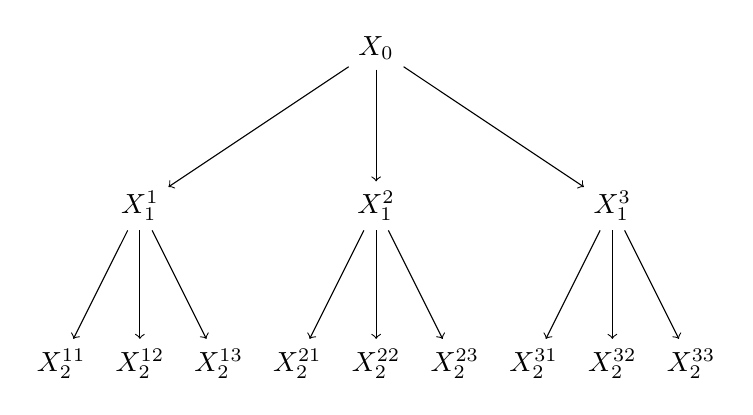
\begin{tikzpicture}
    \draw (5, 4) node[rectangle] (root) {$X_0$};
    
    \foreach \branch in {1,2,3}{
        \draw (3*\branch - 1, 2) node[rectangle] (1\branch) {$X_1^{\branch}$};
        \draw[->] (root) -- (1\branch);
        \foreach \child in {1,2,3}{
            \draw (\child + 3*\branch - 3, 0) node[rectangle] (2\branch\child) {$X_2^{\branch\child}$};
            \draw[->] (1\branch) -- (2\branch\child);
        }
    }


    % \foreach \x in {1,2,3,5}{
    %         \draw[->] (root) -- (1\x);
    % }

    % \foreach \time in {1,2}{
    %     \foreach \x in {1,2,3,5}{
    %         \foreach \target in {1,2,3,5}
    %             \pgfmathtruncatemacro\nexttime{\time+1}
    %             \draw[->] (\time\x) -- (\nexttime\target);
    %     }
    % }

\end{tikzpicture}
\end{document}